\section{Uitvoering en resultaten}
% In dit hoofdstuk wordt de daadwerkelijke uitvoering van de practice based research beschreven, waarbij de in het hoofdstuk methode beschreven aanpak wordt gevolgd. De verhouding tussen praktijk in de vorm van projecten en onderbouwing kan flink uiteenlopen, van 80/20% tot 20/80%. De thesis is daarbij niet alleen een droog projectverslag. De nadruk moet op de verantwoording liggen: reflectie op de relatie tussen de gevolgde aanpak aanpak en resultaten.

\subsection{Onderbouwen aannames}

In dit hoofdstuk ga ik de gemaakte aannames verder beschrijven en beargumenteren.

\subsubsection*{Vernieuwd luistergedrag}

\begin{quotebox}
Door het vernieuwde luistergedrag binnen streamingdiensten heeft het album als distributievorm zijn individuele waarde verloren.
\end{quotebox}
Streamingdiensten zoals Spotify hebben het luistergedrag van mensen merkbaar veranderd. Waar in de tijd van de LP en CD veel werd geluisterd naar albums is deze vorm van publiceren van muziek steeds minder vanzelfsprekend. Muziek wordt nu vaker gepubliceerd als losse nummers (singles), of in de vorm van een EP met 3 a 4 nummers.

Dit heeft meerdere oorzaken: de eerste is dat het via streamingdiensten makkelijker is om losse releases te doen. Er is geen fysiek medium wat gedrukt en geleverd moet worden, maar een online dienst waarbij de content overal tegelijk beschikbaar is. Artiesten hoeven daarom niet meer te wachten tot ze genoeg nummers hebben voor een album, maar kunnen direct een nummer uitbrengen.

Een andere reden is dat de manier waarom mensen muziek vinden is veranderd. Er wordt nu veel meer geluisterd via playlists. Binnen deze playlists is muziek van meerdere artiesten gebundeld met bijvoorbeeld eenzelfde genre. De luisteraar hoeft niet meer zelf op zoek naar nieuwe muziek, maar kan dit overlaten aan de curator van de playlist.

Het is voor de artiest makkelijker om een los nummer te maken dan een heel album. Een album moet een geheel zijn, waarbij de nummers op elkaar aansluiten. Vaak heeft een album een overkoepelend thema, of verteld het een doorlopend verhaal (concept album).

Een album heeft automatisch meer waarde dan een los nummer. Dit komt omdat er meer tijd en moeite in is gestoken. Het is een groter geheel, waarbij de nummers op elkaar aansluiten. Een album is een groter project dan een los nummer. Dit is ook te zien aan de prijs.

Het lijkt er hiermee op dat dit een voordeel is voor beginnende artiesten. Ze kunnen sneller muziek uitbrengen en hoeven niet te wachten tot een album af is. Toch 

\todo{Dit was een braindump, moet nog herschreven worden}
\begin{todolist}
  \item[\done] Beschrijven stelling
  \item[\done] Oorzaken
  \begin{todolist}
    \item[\done] Makkelijker om losse releases te doen
    \item[\done] Muziek wordt gevonden via playlists
  \end{todolist}
  \item Waarom heeft een album meer waarde?
  \item Is het een probleem dat deze verschuiving plaatsvindt?
\end{todolist}

\subsubsection*{Waarde verschoven naar platform}
\begin{quotebox}
De waarde zit op dit moment niet meer in de muziek, maar in het platform dat toegang biedt tot de voor de luisteraar haast onbeperkte hoeveelheid aan content.
\end{quotebox}
\begin{todolist}
  \item Luisteraars betalen niet voor de muziek, maar voor de toegang.
  \item Ze hebben vaak geen idee hoe het geld verdeeld wordt onder de artiesten. Ze willen gewoon muziek luisteren.
  \item Probleem van abonnement: geld gaat in een groot zwart gat
  \item Muziek als identiteit veranderd naar achtergrond
\end{todolist}

\subsubsection*{Waarde zit in community}
\begin{quotebox}
De waarde van muziek zit in de community die wordt gevormd rondom de muziek.
\end{quotebox}
\begin{todolist}
  \item Geen grote fan van één artiest zoals in de '80, maar fan van genre
  \item Sterk genre afhankelijk, sommige genres zijn wel nog erg op fanbase gericht
  \begin{todolist}
    \item Metal
    \item KPop
  \end{todolist}
  \item Merchandise is erg belangrijk bij de communities. Het is een manier om te laten zien dat je bij de community hoort.
  \item Artiesten zijn steeds meer bezig met het opbouwen van een community. Dit doen ze door middel van social media.
\end{todolist}

\subsubsection*{Beginnende artiesten niet rendabel}
\begin{quotebox}
Doordat beginnende artiesten op streamingdiensten direct concurreren met artiesten op professioneel niveau is het moeilijk om door te breken. Dit is slecht voor de diversiteit binnen de muziekindustrie.
\end{quotebox}
\begin{todolist}
  \item Doordat beginnende artiesten niet rendabel zijn is het een grote drempel om volledig (financieel) te focussen op muziek. Hierdoor stoppen veel beginnende artiesten met muziek maken, of brengen ze minder muziek uit.
\end{todolist}

\subsubsection*{Muziek raakt kwijt in geheel}
\begin{quotebox}
Hoewel het steeds makkelijker is om muziek te uploaden, zorgt dit er ook voor dat de muziek kwijtraakt in het grote geheel.
\end{quotebox}
\begin{todolist}
  \item Iedereen kan muziek maken en dit makkelijk uploaden naar streamingdiensten. Hierdoor is er een overvloed aan muziek. Het is moeilijk om op te vallen tussen al deze muziek.
  \item Muzikanten maken muziek waarmee ze makkelijker op playlists komen. Hierdoor wordt er minder geëxperimenteerd met muziek. Resultaat is dat de muziek meer van hetzelfde is.
\end{todolist}

\subsection {Uitwerken businessplan}

Het businessplan is uitgewerkt in een apart document. Dit document is samen met een presentatie voor een pitch te vinden in bijlage \ref{bijlage:businessplan} en \ref{bijlage:pitch}. In dit hoofdstuk zal ik de belangrijkste punten uit het businessplan bespreken.

In het businessplan wordt sterk ingegaan op de verschillende sub-producten van de NichePlayer. Dit is een belangrijk onderdeel van het businessplan omdat de kernfunctie, het afspelen van muziek, een gratis dienst zal zijn. Door de verschillende sub-producten te verkopen kan ik als ontwikkelaar toch geld verdienen en daarmee de NichePlayer blijven door ontwikkelen. De artiest heeft ook een extra gevoel van controle omdat die zelf kan kiezen welke producten en abonnementen worden ingekocht. De inkomsten die ik als bedrijf binnen krijg hebben niets te maken met het geld wat een artiest verdient met de verkoop van zijn muziek.

\subsubsection*{NichePlayer Artist}
Zoals eerder genoemd is dit de kern van de NichePlayer. De NichePlayer Artist kan muziek verkopen, afspelen, het luistergedrag opslaan (voornamelijk voor de verkoop). Er wordt gefocust op controle. De artiest bepaalt het uiterlijk, de content en de functionaliteiten van de NichePlayer.

De reden dat een artiest een NichePlayer wil is omdat de artiest dan meer controle heeft over de muziek en de inkomsten die eruit voortkomen. Daarnaast kan binnen een NichePlayer Artist ook een community ontstaan rond de muziek en de artiest.

\subsubsection*{NichePlayer Hosting}
Uit gesprekken en een enquête in mijn 3e jaars paper van de Bachelor is gebleken dat veel artiesten niet de kennis hebben om een website te hosten. Daarnaast geven artiesten vaak aan zich te willen focussen op de muziek, en niet op randzaken zoals het hosten van een website.

De NichePlayer Hosting Service is voornamelijk bedoeld voor het gemak van de artiest. In plaats van dat de artiest zelf een website moet installeren wordt dit allemaal door de Hosting Service gedaan. Inrichten van de website en het uploaden van de content wordt wel door de artiest gedaan. De websites gehost door de Hosting Service zijn hetzelfde als het de NichePlayer Artist versie, maar dan gehost op een server van NichePlayer.

Het hosten van een website kost geld, zowel voor opslag als bandbreedte van de verbinding. De artiest betaald een vast bedrag per maand voor de hosting van de website. Dit bedrag is afhankelijk van de hoeveelheid opslag en bandbreedte die de artiest nodig heeft. Binnen NichePlayer worden servers aangeschaft en ingericht voor het hosten van de sites. De kosten voor de servers worden gedekt door de maandelijkse betalingen van de artiesten.

\subsubsection*{NichePlayer Extended Services}
De Extended Services zijn extra functionaliteiten die het gebruik van de NichePlayer Artist verder uitbreiden. De Extended Services zijn optioneel en kunnen per functie worden aangeschaft door de artiest.

Veel van deze functies zijn gebaseerd op technische restricties van de manier waarop de NichePlayer Artist is opgezet. Het gaat hierbij om features die niet via een standaard webserver zoals apache server kunnen lopen, of bepaalde software licenties nodig hebben. Hoewel de extended services in theorie zelf te hosten is (via een docker image), vergt dit veel technische kennis. Het is dan ook een goede reden om als ontwikkelaar de extended services apart aan te bieden.

Een van de extended services is een Media Transcoder. Hiermee kan een artiest een enkel hoog kwaliteit bestand uploaden, die vervolgens wordt omgezet naar verschillende kleinere kwaliteiten. Dit is een belangrijke functie voor het gebruiksgemak van luisteraars, omdat zij zo zelf kunnen kiezen welke kwaliteit ze willen luisteren. Grote bestanden kost veel opslag en bandbreedte, wat op mobiele verbindingen veel geld kost. Als een luisteraar echter thuis is, kan die wel de hoogste kwaliteit luisteren.

De Media Transcoder is een complexe functie die veel CPU-kracht en bepaalde programma's  nodig heeft. Het is daarom niet mogelijk om deze functie op een standaard webserver te draaien. De Media Transcoder wordt daarom aangeboden als een Extended Service.

Een andere extended service is Large File Hosting. Dit staat los van de Hosting Service die hiervoor genoemd is. Deze service is bedoeld voor het hosten van grote bestanden zoals verschillende kwaliteiten van mediabestanden. Door deze bestanden los te halen van de NichePlayer Artist kan de website sneller laden en is het zelf-hosten van de website goedkoper.

\subsubsection*{NichePlayer Hub}
Een van de krachtige features van bestaande streamingdiensten is het vinden van nieuwe muziek en content. Dit is tegenwoordig een van de voornaamste redenen dat artiesten hun muziek publiceren op streamingdiensten.

De NichePlayer Hub is een centrale plek waar luisteraars nieuwe muziek kunnen vinden. De Hub verzameld de losse NichePlayer Artist websites en bouwt er een algemene streamingdienst omheen. De muziek is nog steeds gehost op de NichePlayer Artist websites, maar de Hub verzameld de muziek en maakt het vindbaar voor luisteraars.

Gebruikers van de Hub vormen vervolgens ook zelf een grote community. \todo{Schrijven over community}

Om zichtbaar te zijn op de Hub moet een artiest een abonnement hebben. Dit abonnement is een vast bedrag per maand. De kosten voor de servers worden gedekt door de maandelijkse betalingen van de artiesten. Daarnaast kan een artiest extra betalen om te hoger in het zoekalgoritme van de Hub te komen. Dit is een extra inkomstenbron voor de NichePlayer.

\subsubsection*{NichePlayer NFC}
\begin{wrapfigure}{r}{0.25\textwidth}
  \centering
  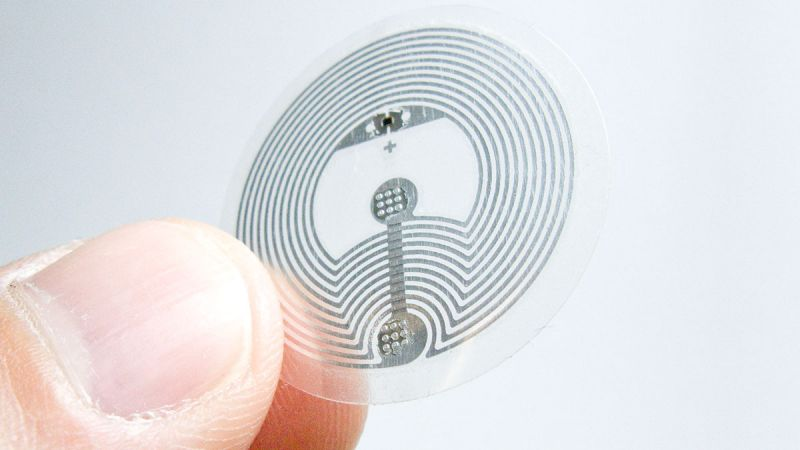
\includegraphics[width=0.25\textwidth]{uitvoering/NFC_chips.jpg}
  \caption{NFC chip}
  \label{fig:uitvoering:NFC_chip}
\end{wrapfigure}
De NFC-feature is een van de killer-features van de NichePlayer. Het is de reden dat een artiest een NichePlayer wil gebruiken. NFC staat voor Near Field Communication. Dit is een techniek die het mogelijk maakt om draadloos informatie uit te wisselen tussen twee apparaten. De meest bekende toepassing van NFC is het contactloos betalen met een pinpas. Binnen de NichePlayer wordt NFC gebruikt om toegang tot de muziek te krijgen. Iedere NFC-chip is uniek, en kan worden gekoppeld aan een album van een NichePlayer Artist. Door een NFC-chip te scannen met een telefoon wordt de toegang gekoppeld met het account van de gebruiker. De gebruiker kan vervolgens de muziek luisteren op alle apparaten die zijn gekoppeld aan het account.

Wanneer een andere telefoon de NFC-chip scant, wordt ook deze gekoppeld aan het account. Dit kan worden gebruikt om de muziek te delen met vrienden. Er zit echter wel een limiet op het aantal accounts dat gekoppeld kan worden aan een chip. Dit is om te voorkomen dat een gebruiker een chip kan kopen en deze vervolgens kan delen met iedereen. De limiet is in te stellen door de artiest, maar zal standaard ingesteld zijn op 3 gebruikers. Wanneer de limiet is bereikt wordt de gebruiker die als eerste gescand heeft ontkoppeld.

Een groot verschil met bestaande distributie media is dat de chip slechts een doorgeefluik is. De muziek wordt niet opgeslagen op de chip, maar op de servers van de artiest. Dit betekent dat de muziek altijd up-to-date is, en dat de artiest de muziek kan aanpassen zonder dat de chip opnieuw gemaakt hoeft te worden. Content is daarnaast ook niet gelimiteerd tot muziek, ook andere media zoals video's en foto's zijn mogelijk. De NichePlayer NFC chips zijn daarom een goede vervanger voor de huidige distributie media.

De NFC-chips maken het mogelijk om muziek op een fysieke wijze te verkopen, maar tijdens het afspelen de voordelen van streaming te hebben. De chips zijn makkelijk te verwerken in bestaande producten als Vinyl platen, CD's en posters, maar bieden meer creativiteit. Daarnaast zijn de chips relatief goedkoop te produceren.

\subsubsection*{NichePlayer Custom development}
Er zijn nog veel meer functionaliteiten te bedenken die de NichePlayer kan bieden. De NichePlayer is een framework, en kan dus worden uitgebreid met nieuwe functionaliteiten. Deze functionaliteiten kunnen worden aangevraagd door middel van offerte bij de ontwikkelaar van de NichePlayer. Hiermee blijft de NichePlayer groeien en kan het worden aangepast aan de wensen van de artiesten.

\subsection {Uitwerken Software}
\subsubsection*{U.F.O.-App}
Ik ben al jaren een framework aan het ontwikkelen waarmee ik snel web-systemen kan opzetten. Dit framework heeft veel verschillende iteraties gezien (begonnen als puur zelf ontwikkeld, nu gebaseerd op verschillende andere libraries). Om de meest recente versie van het framework te testen ben ik de afgelopen 1.5 jaar bezig geweest met het ontwikkelen van een dranksysteem app voor mijn studentenscouting groep de U.F.O.-Stam uit Utrecht. Het concept achter de app heeft verder weinig te maken met de opleiding (verkopen van drankjes en andere producten tijdens de opkomsten). Wat wel relevant is voor de NichePlayer, zijn onderdelen zoals user-authenticatie, media upload en transcodering, User Interface en User Experience design en algehele stabiliteit van het systeem. Met andere woorden, de app is een goede test-case voor het ontwikkelen van de kern van het framework.

Het grote voordeel van het ontwikkelen van deze app voor mijn scoutinggroep is dat ik het framework heb kunnen testen in een realistische live omgeving. Hoewel er in iets meer dan een jaar tijd meer dan 5000 transacties zijn gemaakt met een totale waarde van meer dan €4800,- was het toegestaan om fouten te maken. De app is niet bedoeld voor commerciële doeleinden en de gebruikers zijn bekend met het feit dat het een ontwikkel project is. Dit heeft mij de mogelijkheid gegeven om het framework te testen in een realistische omgeving, zonder dat er grote gevolgen waren als er iets fout ging.

De app is inmiddels stabiel en heeft meer dan 100 gebruikers. Op piekmomenten wordt de app door meer dan 50 mensen tegelijk gebruikt, wat niet mogelijk was met oude versies van het framework tijdens mijn bachelor uitwerking van de NichePlayer.

\subsubsection*{Plugins}
Tijdens de laatste update aan de U.F.O.-App heb ik kern onderdelen van het framework verplaatst naar losse plugins en GIT repositories. Hierbij gaat het onder andere om de API-communicatie, gebruiker authenticatie, media-upload en enkele UI elementen die ik vaak hergebruik. Ik realiseerde mij dat ik deze onderdelen vaak ontwikkel in verschillende projecten, maar iedere keer vanaf scratch begin. Door deze onderdelen te verplaatsen naar losse plugins kan ik ze makkelijk hergebruiken in andere projecten. Dit is ook het geval bij de NichePlayer. De NichePlayer maakt gebruik van verschillende plugins die ik heb ontwikkeld voor de U.F.O.-App. Het grote voordeel van deze plugin-structuur is dat de projecten profiteren van elkaars ontwikkeling. Als ik een update ontwikkel voor de U.F.O.-App, kan ik deze ook vrijwel direct gebruiken in de NichePlayer. Dit zorgt ervoor dat ik sneller kan ontwikkelen en meer kan focussen op de implementatie van de unieke functies van de verschillende systemen, in plaats van de kern van het systeem.

\subsubsection*{API-communicatie}
De NichePlayer maakt gebruik van een API om te communiceren tussen de frontend en de backend. Deze API was in vorige versies van mijn framework gebaseerd op GraphQL. Deze api-vorm gebruikt een enkele endpoint (url) waarnaar een zogenaamde query (een vraag of opdracht) wordt gestuurd. Deze query wordt vervolgens verwerkt door de server en het resultaat wordt teruggestuurd naar de client. Het grote voordeel van GraphQL is dat de client zelf kan bepalen welke data hij nodig heeft. Hierdoor kan de server efficiënter werken en hoeft er minder data over verschillende requests verstuurd te worden. Ingewikkelde en uitgebreide zoekopdrachten zoals "geef mij een album met alle nummers en artiesten, en alle gebruikers die op dit moment naar dit album aan het luisteren zijn" kan in een enkele query verstuurd worden.

GraphQL bleek echter verschillende nadelen te hebben binnen deze uitwerking van het systeem. Zo was het bijvoorbeeld niet mogelijk om queries te cachen en hergebruiken voor verschillende users. Het grootste nadeel was echter een gebrek aan configuratie aan de frontend kant. Ik gebruikte een library die de queries voor mij genereerde, maar deze library bleek niet intelligent of aanpasbaar genoeg. Hierdoor was het niet mogelijk om de queries te optimaliseren voor de verschillende functies van de app. Een voorbeeld was een circulaire referentie die moeilijk op te lossen was. Bij deze circulaire referentie vroeg ik bijvoorbeeld een om een album, waarbij ik automatisch alle tracks van het album mee kreeg. Een track had echter ook een lijst van gebruikers die recent naar dat nummer hadden geluisterd. Deze gebruikers hadden vervolgens weer een lijst van albums die ze hadden gekocht, waarbij ik weer alle tracks van het album kreeg. Dit zorgde ervoor dat de app onnodig veel data moest verwerken en versturen. De cirkel was enkel te doorbreken door het automatisch ophalen van relaties uit te zetten, of handmatig de queries te schrijven in plaats van te laten genereren door de library. Hiermee ging de kracht van het gebruik van de GraphQL library verloren, waardoor het toch makkelijker was om over te stappen naar eenvoudigere API vormen.

De nieuwe API is gebaseerd op REST. Dit is een meer traditionele API-vorm waarbij er verschillende endpoints zijn op de server die verschillende data terugsturen. Het grote voordeel van deze API-vorm is dat het makkelijker is om de data te optimaliseren voor de verschillende functies van de app. Zo kan ik bijvoorbeeld een endpoint maken die enkel de data terugstuurt die nodig is voor het afspelen van een album, en een andere endpoint die voor de administrator van het systeem juist alle data doorstuurt. Dit zorgt ervoor dat de app sneller werkt en minder data hoeft te versturen. De REST-API is meer configuratie werk, maar zorgt voor overzichtelijkere code en een snellere app.

Een voordeel van REST is dat ik de API kan hergebruik tussen verschillende programmeertalen. De NichePlayer-Artist moet vanwege zijn self-hostable karakter geschreven worden in PHP, terwijl de NichePlayer-Hub geschreven wordt in RubyOnRails. Beide programmeertalen hebben een eigen manier van communiceren met een API, maar door de API te schrijven in een taalonafhankelijke syntax kan ik de API hergebruiken in beide projecten.

\subsubsection*{NichePlayer-Artist}
Na lang te hebben gewerkt aan de U.F.O.-App was het tijd om de vertaalslag te maken naar de NichePlayer-Artist. Omdat ik in de laatste updates aan de U.F.O.-App had gewerkt met plugins kon ik in erg korte tijd de code strippen en herschrijven. Ik ben uiteindelijk ongeveer 2 dagen bezig geweest met het strippen van de code van het dranksysteem, en vervolgens een dag of 3 met het implementeren van de Minimal Viable Product eisen van de NichePlayer. Dit laatste was voornamelijk mogelijk door het hergebruiken van code van mijn bachelor versie van de NichePlayer en kennis die ik de afgelopen jaren heb opgedaan als developer bij TapTapes.

% \subsection*{OUTLINE}
% In dit hoofdstuk wordt verslag gegeven van het proces van het onderzoek. Het businessplan zal hier worden uitgewerkt en onderbouwd. Daarnaast zal het ook worden gebruikt om het prototype te kunnen realiseren en testen bij een testpubliek. Dit testen zal worden geprobeerd te doen tijden tijdens het onderzoek, maar dat is afhankelijk van de beschikbare tijd.
